% The entire content of this work (including the source code
% for TeX files and the generated PDF documents) by 
% Hongxiang Chen (nicknamed we.taper, or just Taper) is
% licensed under a 
% Creative Commons Attribution-NonCommercial-ShareAlike 4.0 
% International License (Link to the complete license text:
% http://creativecommons.org/licenses/by-nc-sa/4.0/).
\documentclass{article}

% My own physics package
% The following line load the package xparse with additional option to
% prevent the annoying warnings, which are caused by the package
% "physics" loaded in package "physicist-taper".
\usepackage[log-declarations=false]{xparse}
\usepackage{physicist-taper}


\makenomenclature % For an index of symbols.

% Show the keys for labels, replace options with "final" when done
% with editing.
\usepackage[draft,notref]{showkeys}

\title{Notes of Topological Transition in a Non-Hermitian Quantum Walk}
\date{\today}
\author{Taper}


\begin{document}


\maketitle
\abstract{
As suggested by the title.
}
\tableofcontents
\section{General}
\label{sec:General}

This paper discusses in general a model charaterised by the follwoing
picture
\begin{figure}[H]
    \centering
    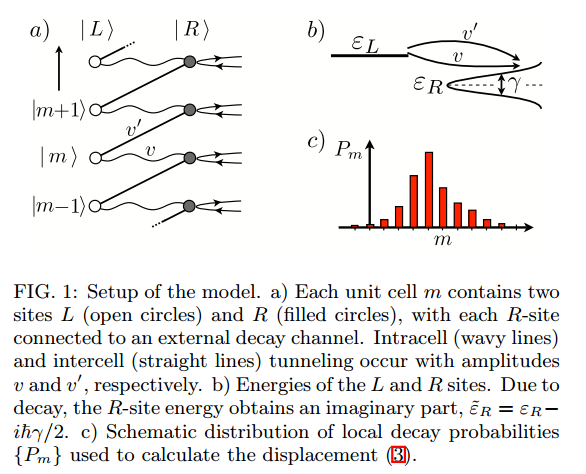
\includegraphics[width=0.8\linewidth]{pics/setup.PNG}
    \caption{Setup}
\end{figure}
The equation of motion is
\begin{align}
    i\hbar \dot{\psi}^L_m = \varepsilon_L\psi^L_m + v\psi^R_m
    +v'\psi^R_{m+1} \\
    i\hbar \dot{\psi}^R_m = \tilde{\varepsilon}_R\psi^R_m + v\psi^L_m
    +v'\psi^L_{m-1}
\end{align}

where
\begin{equation}
    \tilde\varepsilon_R = \varepsilon_R - i\hbar \gamma/2
\end{equation}

\subsection{I can get}
\label{sec:I-can-get}

\begin{equation}
    \ket{\psi} = \sum_m \ket{\psi_m^L} + \ket{\psi_m^R}
\end{equation}
\begin{equation}
    \frac{\partial }{\partial t}\braket{\psi|\psi}
    = -\sum_m \gamma \braket{\psi^R_m|\psi^R_m}
\end{equation}
(All leakage from "R" site!)
(draft page 1 to 2)

\colorbox{red}{Strange:}
\begin{equation}
    \sum_m P_m = 1
\end{equation} (draft page 3)
\subsection{Result}
\label{sec:Result}

\begin{myquote} \enquote{
we find that the average displacement
of the particle during the course of its decay, $\Delta m =\sum_m mP_m$, 
is exactly quantized as an integer (0 or 1 unit
cells), where $P_m$ is the probability distribution for decay from
different sites.

As in the case of
the quantum Hall conductance, this quantization results
from an underlying topological structure; in this case it
is the winding number of the relative phase between two
components of the Bloch wave function.

Using the topological origin of this phenomenon, we are able to show
that the quantization is insensitive to parameters and is
robust against certain types of noise and decoherence.

The topological transition, which is accompanied by the formation of
a non-decaying dark state, leads to a prediction of threshold-like
pumping of nuclear polarization, along with strong suppression of
current due to the divergence of dwell time at the threshold
} \end{myquote}

\begin{myquote} \enquote{
our motivation is to provide a simple
model of nuclear spin pumping in spin-blockaded double
quantum dots [9, 10, 11] in the presence of competing
effects of the hyperfine and spin-orbital interactions, as
in Ref.[11].
} \end{myquote}
\section{Anchor}
\label{sec:Anchor}

\begin{thebibliography}{1}
    \bibitem{1dwalk} Topological Transition in a Non-Hermitian Quantum
    Walk,
    \href{https://arxiv.org/ct?url=http%3A%2F%2Fdx.doi.org%2F10%252E1103%2FPhysRevLett%252E102%252E065703&v=f6968ad6}{arXiv}
\end{thebibliography}
\printnomenclature
\section{License}
The entire content of this work (including the source code
for TeX files and the generated PDF documents) by 
Hongxiang Chen (nicknamed we.taper, or just Taper) is
licensed under a 
\href{http://creativecommons.org/licenses/by-nc-sa/4.0/}{Creative 
Commons Attribution-NonCommercial-ShareAlike 4.0 International 
License}. Permissions beyond the scope of this 
license may be available at \url{mailto:we.taper[at]gmail[dot]com}.
\end{document}
